\documentclass[12pt]{standalone}
\usepackage{tikz}
\begin{document}
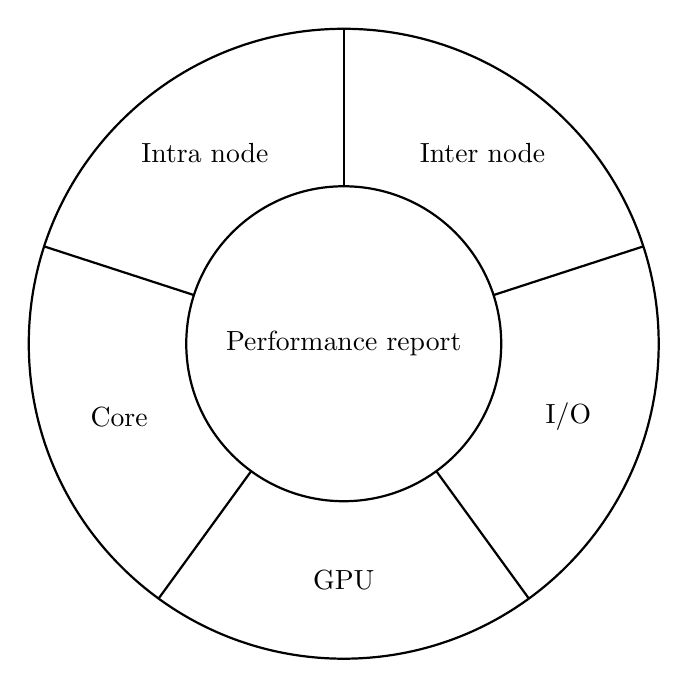
\begin{tikzpicture}
    \draw[thick] (0,0) circle (4.0);
    \draw[thick] (0,0) circle (2.0);
    \foreach \a in {18,90,162,234,306}
        \draw[thick] (\a:2.) -- (\a:4.0);
    \draw (0: 0) node {Performance report};
    \draw (54: 3.0) node {Inter node};
    \draw (126: 3.0) node {Intra node};
    \draw (198: 3.0) node {Core};
    \draw (270: 3.0) node {GPU};
    \draw (342: 3.0) node {I/O};
\end{tikzpicture}
\end{document}
